\documentclass[journal,onecolumn]{IEEEtran}

\usepackage[T1]{fontenc}
\usepackage[utf8]{inputenc}
\usepackage{graphicx}
\usepackage{amsmath,amssymb}
\usepackage{booktabs}
\usepackage{multirow}
\usepackage{subcaption}
\usepackage{listings}
\usepackage{xcolor}
\usepackage{url}

\lstdefinestyle{pycode}{
  language=Python,
  basicstyle=\ttfamily\small,
  keywordstyle=\color{blue!70!black},
  commentstyle=\color{green!40!black},
  stringstyle=\color{red!60!black},
  showstringspaces=false,
  breaklines=true,
  frame=single,
  tabsize=4
}

\title{Distributed Viewpoint-Level Traffic Analytics over UVH-26: \\
Architecture, Distributed Processing Strategy, and Interactive Insight Layer}

\author{Dhrusheek Rishi Menon, Nethi Kushala Kumar, Rishinath Kurup, Yalamanchi Kushal}

\begin{document}

\maketitle

\begin{center}
\textbf{Group 8 --- Case Study on Apache Spark with Application on City-Wide Analytics}\\[4pt]
\textbf{Dhrusheek Rishi Menon} --- CB.SC.U4CSE23716\\[2pt]
\textbf{Nethi Kushala Kumar} --- CB.SC.U4CSE23735\\[2pt]
\textbf{Rishinath Kurup} --- CB.SC.U4CSE23741\\[2pt]
\textbf{Yalamanchi Kushal} --- CB.SC.U4CSE23766\\[6pt]
\textbf{GitHub Repository: \url{https://github.com/not-good-keeper/DS-City-Analytics}}
\end{center}

\begin{abstract}
This document provides a detailed single-column IEEE-style technical account of a distributed systems project for city traffic analytics over UVH-26. The pipeline is organized into three stages: deterministic viewpoint reconstruction, distributed Spark-based analytics, and a dashboard-based interpretation layer. The central systems contribution is a distribution-aware transformation of Stage 1 image-to-viewpoint mappings into grouped viewpoint workloads and node-bucket assignments suitable for parallel execution. Stage 2 integrates Spark DataFrame transformations, schema normalization of COCO-formatted annotations, controlled shuffles, broadcast joins, entropy-based class uncertainty scoring, and congestion synthesis through compound metrics. The resulting full artifact contains 4,780 viewpoint records derived from 26,646 mapped images and 316,220 joined annotation rows. The report emphasizes distributed execution semantics, partition behavior, computational hierarchy, metric derivation, reproducibility pathways, and code-level implementation details. A set of dataset sample images and dashboard snapshots is included to connect distributed processing outputs to real traffic-scene interpretation tasks.
\end{abstract}

\begin{IEEEkeywords}
Distributed systems, Apache Spark, Spark Standalone, traffic analytics, UVH-26, COCO annotations, entropy, congestion index, viewpoint analytics, data engineering.
\end{IEEEkeywords}

\section{Introduction}

Urban traffic understanding at scale requires more than object detection outputs and ad hoc scripts. Image collections in practical deployments contain large object counts, camera diversity, category imbalance, and annotation noise. As a result, viewpoint-centric aggregation and robust runtime orchestration become mandatory for obtaining reproducible intelligence.

The implemented project addresses this requirement by combining: (1) deterministic viewpoint reconstruction from image streams, (2) distributed statistical aggregation in Apache Spark, and (3) an interactive analytics interface for interpretation and verification. The design objective is not solely computational speed; the objective is a complete distributed analytics lifecycle where data contracts, transformations, metrics, and outputs remain auditable and extensible.

In distributed systems terms, the project models the analytics workflow as a hierarchy of transformations over partitioned datasets. Low-level image and annotation records are transformed into per-image metrics, then folded into viewpoint-level summaries through distributed reductions. The final layer exposes these summaries for human-in-the-loop analysis.

\section{Problem Statement and Distributed Requirements}

\subsection{Formal Problem Context}
Given:
\begin{itemize}
    \item A mapping $M = \{(i, v)\}$ where image $i$ belongs to viewpoint $v$,
    \item COCO-style annotations containing image metadata, object categories, and per-instance bounding boxes,
\end{itemize}
the system must generate viewpoint-level traffic descriptors that are robust, interpretable, and scalable under distributed execution.

\subsection{Distributed Requirements}
The following requirements define the distributed systems scope:
\begin{enumerate}
    \item \textbf{Partition-aware processing:} Large annotation tables must be processed through distributed joins and grouped reductions.
    \item \textbf{Load balancing:} Viewpoints with highly variable image counts must be assigned across node buckets to reduce straggler risk.
    \item \textbf{Reproducibility:} Smoke-to-full workflows must preserve schema consistency and metric semantics.
    \item \textbf{Observability:} Logs must expose master mode, parallelism, shuffle partitions, row counts, and runtime durations.
    \item \textbf{Interpretability:} Metrics should support both ranking and explanation, not only scalar performance summaries.
\end{enumerate}

\section{System Architecture (Hierarchical View)}

\subsection{Stage 1: Viewpoint Reconstruction Layer}
Stage 1 outputs a deterministic CSV mapping between image identifiers and inferred viewpoint identifiers. This stage creates the semantic bridge between raw camera frames and viewpoint-level analytics.

\subsection{Stage 2: Distributed Analytics Layer}
Stage 2 is implemented in \texttt{spark\_jobs/analytics\_job.py}. Core operations include:
\begin{enumerate}
    \item Parsing Stage 1 mapping and COCO train/val JSON files,
    \item Normalizing nested image and annotation arrays,
    \item Joining annotations with image metadata and viewpoint mapping,
    \item Computing per-image signals (count, area, density),
    \item Computing per-viewpoint aggregate metrics,
    \item Serializing full metrics into JSONL output.
\end{enumerate}

\subsection{Stage 3: Insight Interface Layer}
Stage 3 in \texttt{stage3/dashboard\_app.py} loads Stage 2 JSONL output into a visual analytics interface. KPI cards, ranking charts, composition plots, and deep-dive views provide human-readable interpretation of distributed outputs.

\subsection{End-to-End Hierarchy}
The architecture can be viewed as a four-level hierarchy:
\begin{itemize}
    \item \textbf{L0 Raw data}: UVH-26 images and COCO annotation documents,
    \item \textbf{L1 Relational normalization}: exploded records with stable join keys,
    \item \textbf{L2 Distributed feature synthesis}: viewpoint-level metrics via Spark shuffles,
    \item \textbf{L3 Analytical interpretation}: interactive exploration and ranking in Stage 3.
\end{itemize}

\section{Distribution-Aware Mapping Transformation}

\subsection{Why Transformation Is Needed}
Image-to-viewpoint pairs are semantically sufficient but operationally inefficient for node-level scheduling. Distributed execution benefits from viewpoint-grouped structures because all image records for a viewpoint are logically co-analyzed.

\subsection{Generated Mapping Artifacts}
The helper script \texttt{spark\_jobs/build\_viewpoint\_mapping.py} produces:
\begin{itemize}
    \item \texttt{viewpoint\_to\_images.jsonl},
    \item \texttt{viewpoint\_to\_images.csv},
    \item \texttt{viewpoint\_bucket\_assignment.csv},
    \item \texttt{bucket\_summary.csv}.
\end{itemize}

\subsection{Bucket Assignment Strategy}
Viewpoints are sorted by descending image cardinality and greedily assigned to the currently lightest bucket. This strategy approximates balanced load allocation in $O(V\log V)$ sorting time plus linear assignment, where $V$ denotes number of viewpoints.

\begin{lstlisting}[style=pycode,caption={Node-bucket assignment logic used for balanced viewpoint distribution.}]
viewpoints_by_size = sorted(grouped.items(), key=lambda kv: len(kv[1]), reverse=True)
buckets = [{"bucket_id": b, "image_count": 0, "viewpoints": []}
           for b in range(num_buckets)]

for viewpoint_id, image_ids in viewpoints_by_size:
    target_bucket = min(buckets, key=lambda x: x["image_count"])
    target_bucket["viewpoints"].append(int(viewpoint_id))
    target_bucket["image_count"] += len(image_ids)
\end{lstlisting}

This mapping-level balancing is important because skew in viewpoint cardinality can produce long-tail stage completion times in distributed group-by workloads.

\section{Distributed Stage 2 Pipeline: Detailed Explanation}

\subsection{Runtime Bootstrap and Spark Controls}
The engine exposes configurable runtime parameters for distributed behavior:
\begin{itemize}
    \item \texttt{--master} for Spark master URI (
    e.g., \texttt{spark://host:7077}),
    \item \texttt{--shuffle-partitions},
    \item \texttt{--default-parallelism},
    \item \texttt{--skip-output-write} for compute-only validation,
    \item \texttt{--preview-jsonl} for deterministic sample export.
\end{itemize}

\begin{lstlisting}[style=pycode,caption={Spark session configuration for distributed execution semantics.}]
builder = SparkSession.builder.appName(args.app_name)
if args.master:
    builder = builder.master(args.master)
builder = builder.config("spark.sql.shuffle.partitions", str(args.shuffle_partitions))
builder = builder.config("spark.default.parallelism", str(args.default_parallelism))
builder = builder.config("spark.sql.adaptive.enabled", "true")
spark = builder.getOrCreate()
\end{lstlisting}

\subsection{Schema Normalization Hierarchy}
The COCO JSON payload is transformed into three normalized relations:
\begin{enumerate}
    \item \textbf{Images relation}: image size and filename-derived image key,
    \item \textbf{Annotations relation}: category references and bounding-box area,
    \item \textbf{Categories relation}: category ID to category name map.
\end{enumerate}

Filename stem extraction standardizes image identifiers before joins. This prevents silent key mismatch between mapping CSV rows and COCO image metadata.

\subsection{Join Design}
The distributed join chain is:
\begin{equation}
J = A \Join I \Join B(M) \Join C
\end{equation}
where:
\begin{itemize}
    \item $A$ = annotation records,
    \item $I$ = image metadata,
    \item $B(M)$ = broadcasted mapping table,
    \item $C$ = categories.
\end{itemize}

Broadcasting $M$ reduces expensive cluster-wide shuffle for the mapping side and is aligned with Spark SQL join tuning recommendations.

\subsection{Per-Image Intermediate Aggregation}
For each pair $(v, i)$ where viewpoint is $v$ and image is $i$:
\begin{align}
\text{vehicle\_count}_{v,i} &= \#\text{annotations in }(v,i) \\
\text{bbox\_density}_{v,i} &= \frac{\sum \text{bbox\_area}_{v,i}}{\text{image\_area}_{i}}
\end{align}

Additional counters classify heavy and two-wheeler detections through keyword grouping.

\subsection{Per-Viewpoint Distributed Reduction}
Per-viewpoint metrics are generated by distributed \texttt{groupBy(viewpoint\_id)} operations.

\begin{align}
\text{total\_images}(v) &= \sum_{i \in v} 1 \\
\text{total\_vehicles}(v) &= \sum_{i \in v} \text{vehicle\_count}_{v,i} \\
\text{avg\_vehicle\_count}(v) &= \frac{\text{total\_vehicles}(v)}{\text{total\_images}(v)} \\
\text{avg\_bbox\_density}(v) &= \frac{1}{N_v} \sum_{i \in v} \text{bbox\_density}_{v,i}
\end{align}

\subsection{Entropy and Congestion Synthesis}
Class distribution probabilities are derived per viewpoint and entropy is computed using base-2 logarithms:
\begin{equation}
H(v) = -\sum_{c\in C} p(c|v)\log_2 p(c|v)
\end{equation}

Congestion index is defined as:
\begin{equation}
\text{congestion\_index}(v) = \text{avg\_vehicle\_count}(v) \times \text{avg\_bbox\_density}(v)
\end{equation}

\begin{lstlisting}[style=pycode,caption={Entropy and congestion implementation segment from Stage 2 analytics engine.}]
entropy_df = class_probs.withColumn(
    "entropy_component",
    F.when(F.col("class_prob") > 0,
           -F.col("class_prob") * F.log2(F.col("class_prob")))
     .otherwise(F.lit(0.0))
).groupBy("viewpoint_id").agg(F.sum("entropy_component").alias("entropy"))

result = viewpoint_core.join(entropy_df, on="viewpoint_id", how="left") \
    .withColumn("congestion_index",
                F.col("avg_vehicle_count") * F.col("avg_bbox_density"))
\end{lstlisting}

\section{Dataset Samples for Contextual Interpretation}

Figure~\ref{fig:uvh26_samples} includes four representative UVH-26 samples used to ground the analytics context in real traffic scenes.

\begin{figure}[!t]
    \centering
    \begin{subfigure}[b]{0.48\textwidth}
        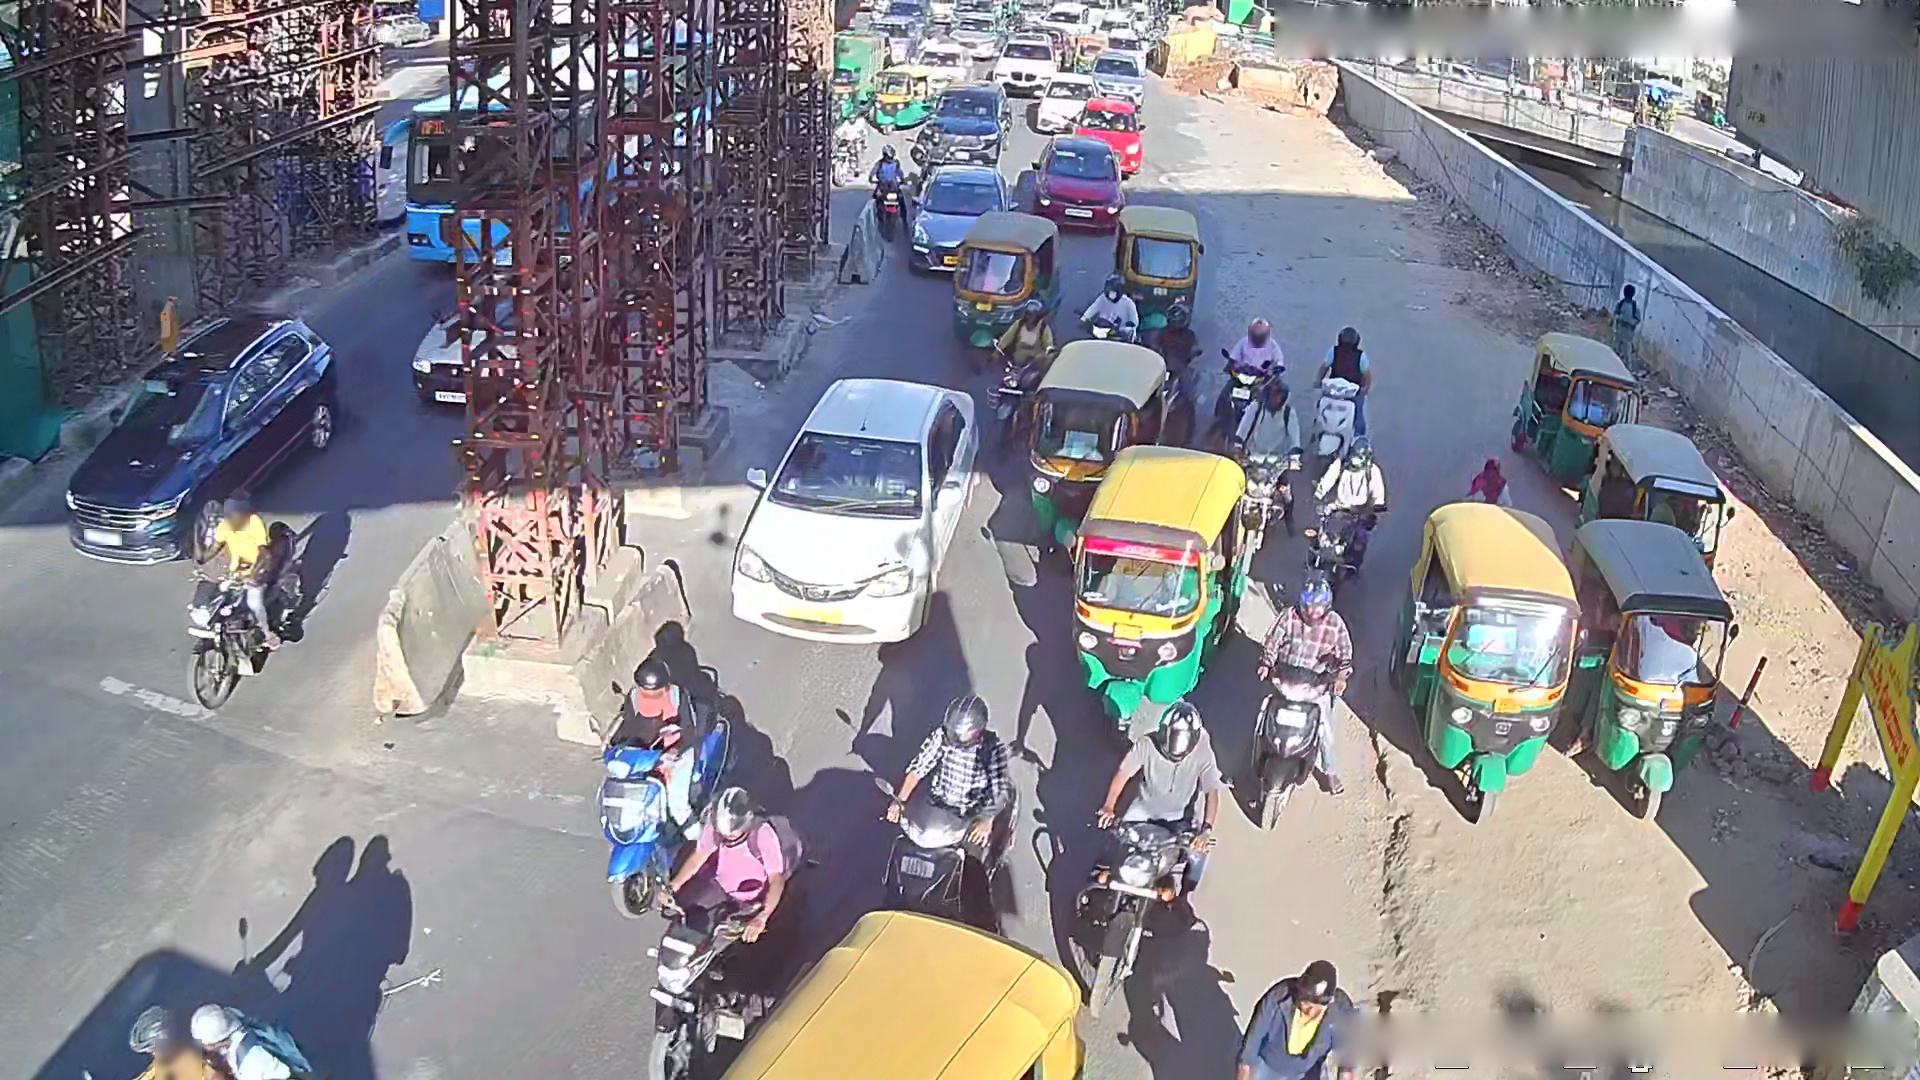
\includegraphics[width=\textwidth]{docs/assets/report/uvh26_train_sample_a.png}
        \caption{Train sample A}
    \end{subfigure}
    \hfill
    \begin{subfigure}[b]{0.48\textwidth}
        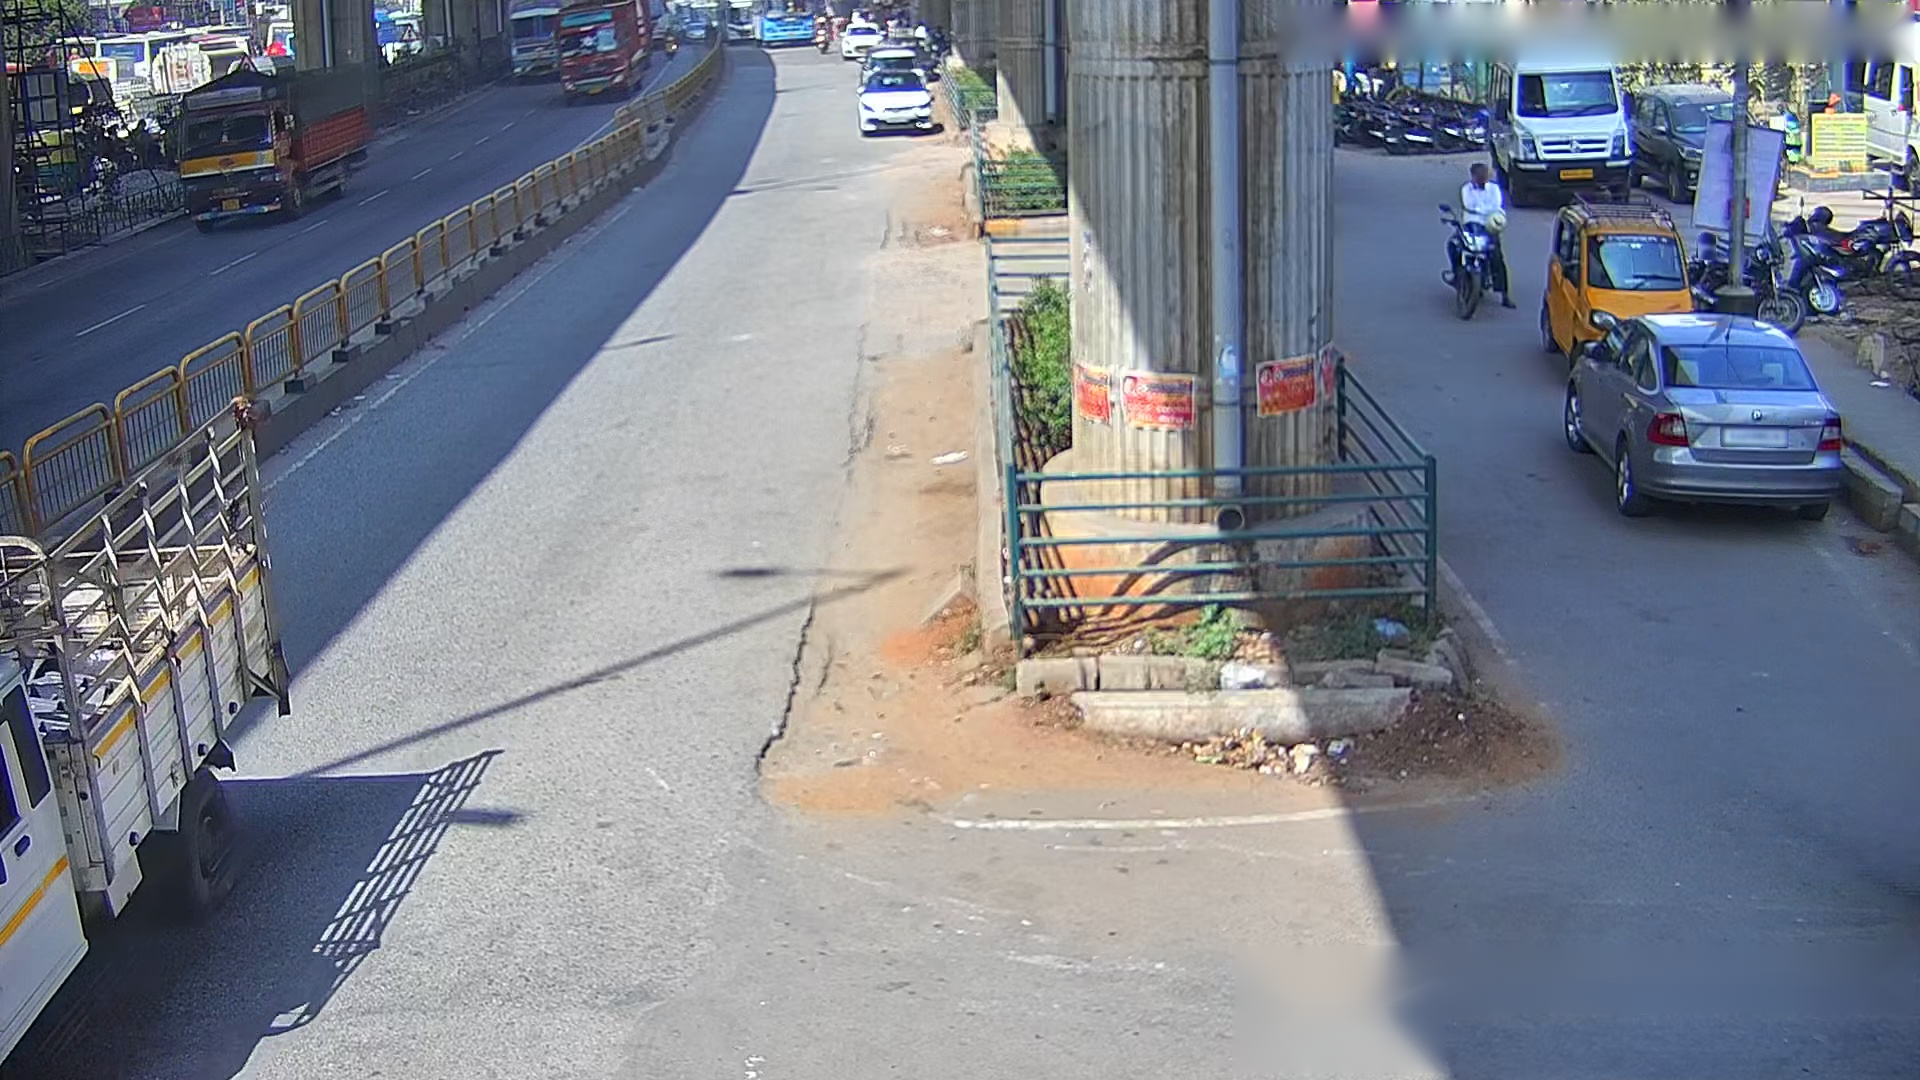
\includegraphics[width=\textwidth]{docs/assets/report/uvh26_train_sample_b.png}
        \caption{Train sample B}
    \end{subfigure}

    \vspace{0.5em}

    \begin{subfigure}[b]{0.48\textwidth}
        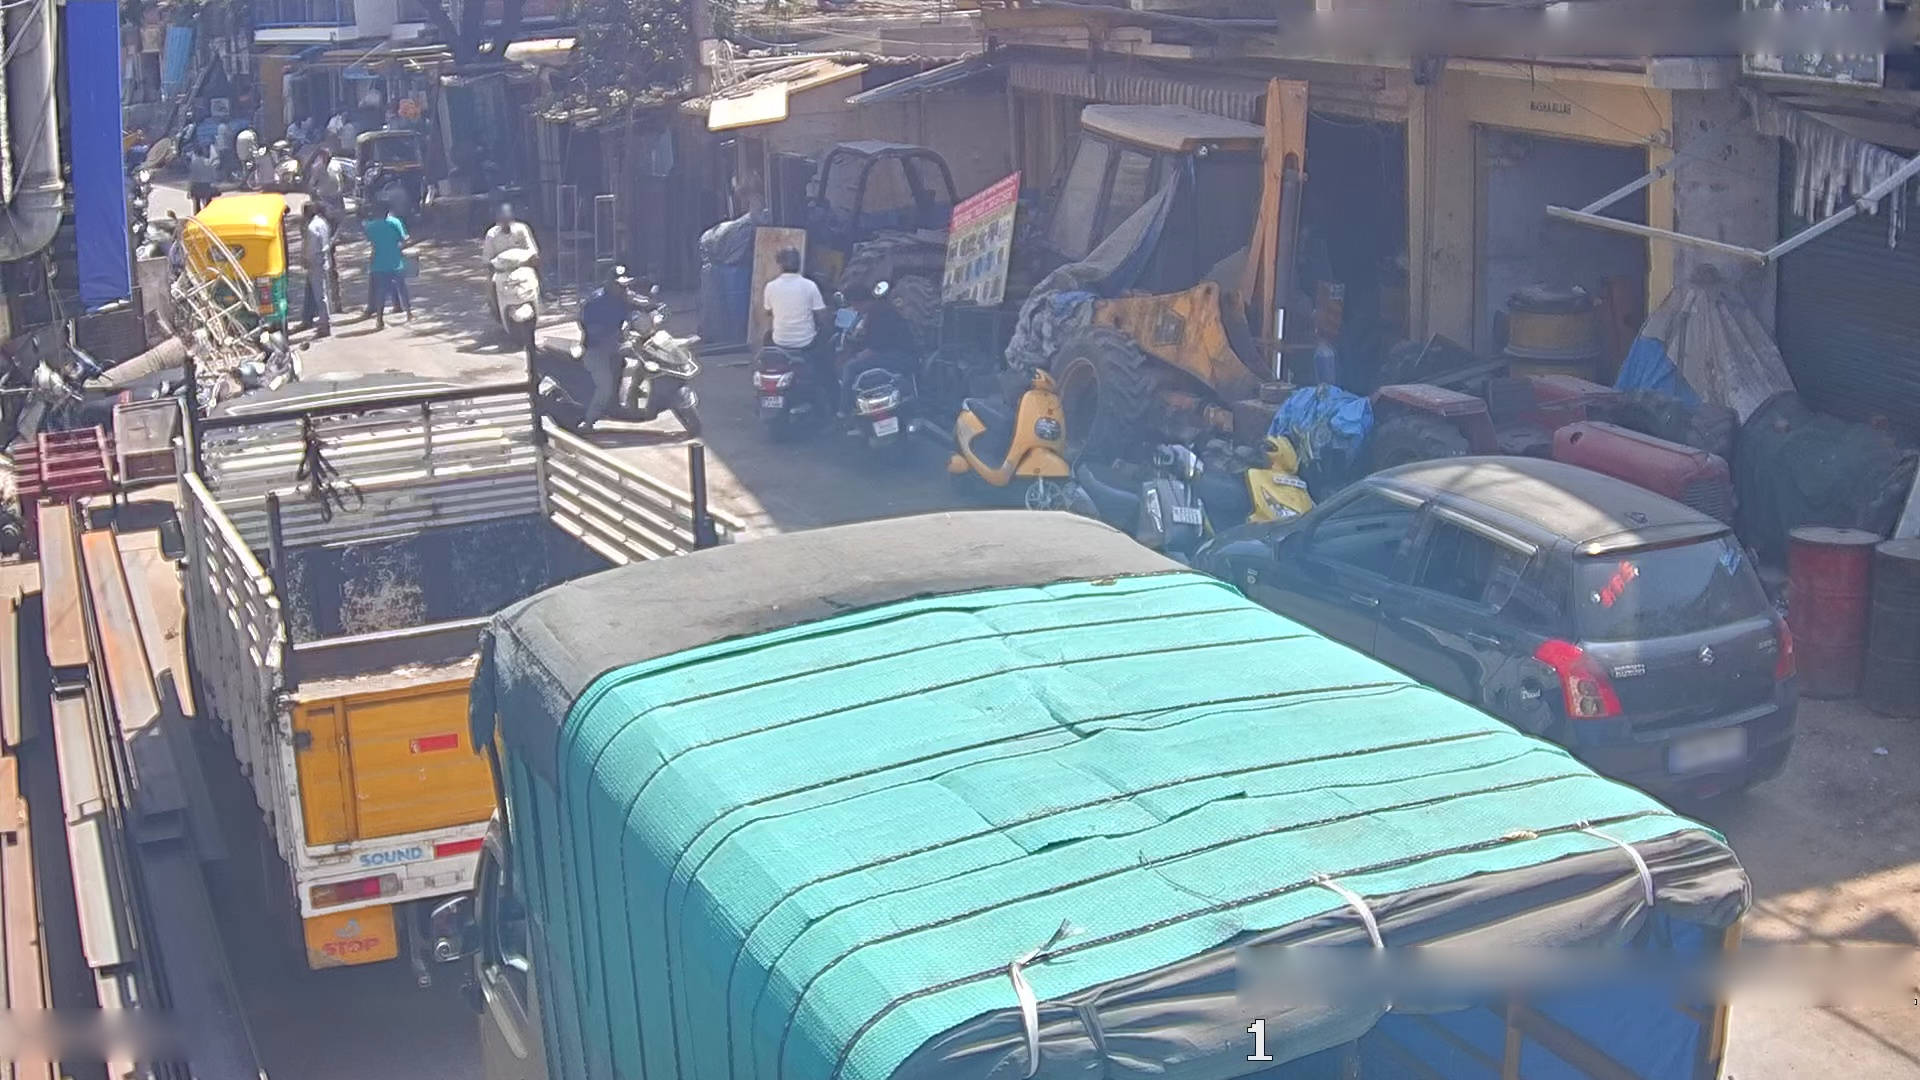
\includegraphics[width=\textwidth]{docs/assets/report/uvh26_train_sample_c.png}
        \caption{Train sample C}
    \end{subfigure}
    \hfill
    \begin{subfigure}[b]{0.48\textwidth}
        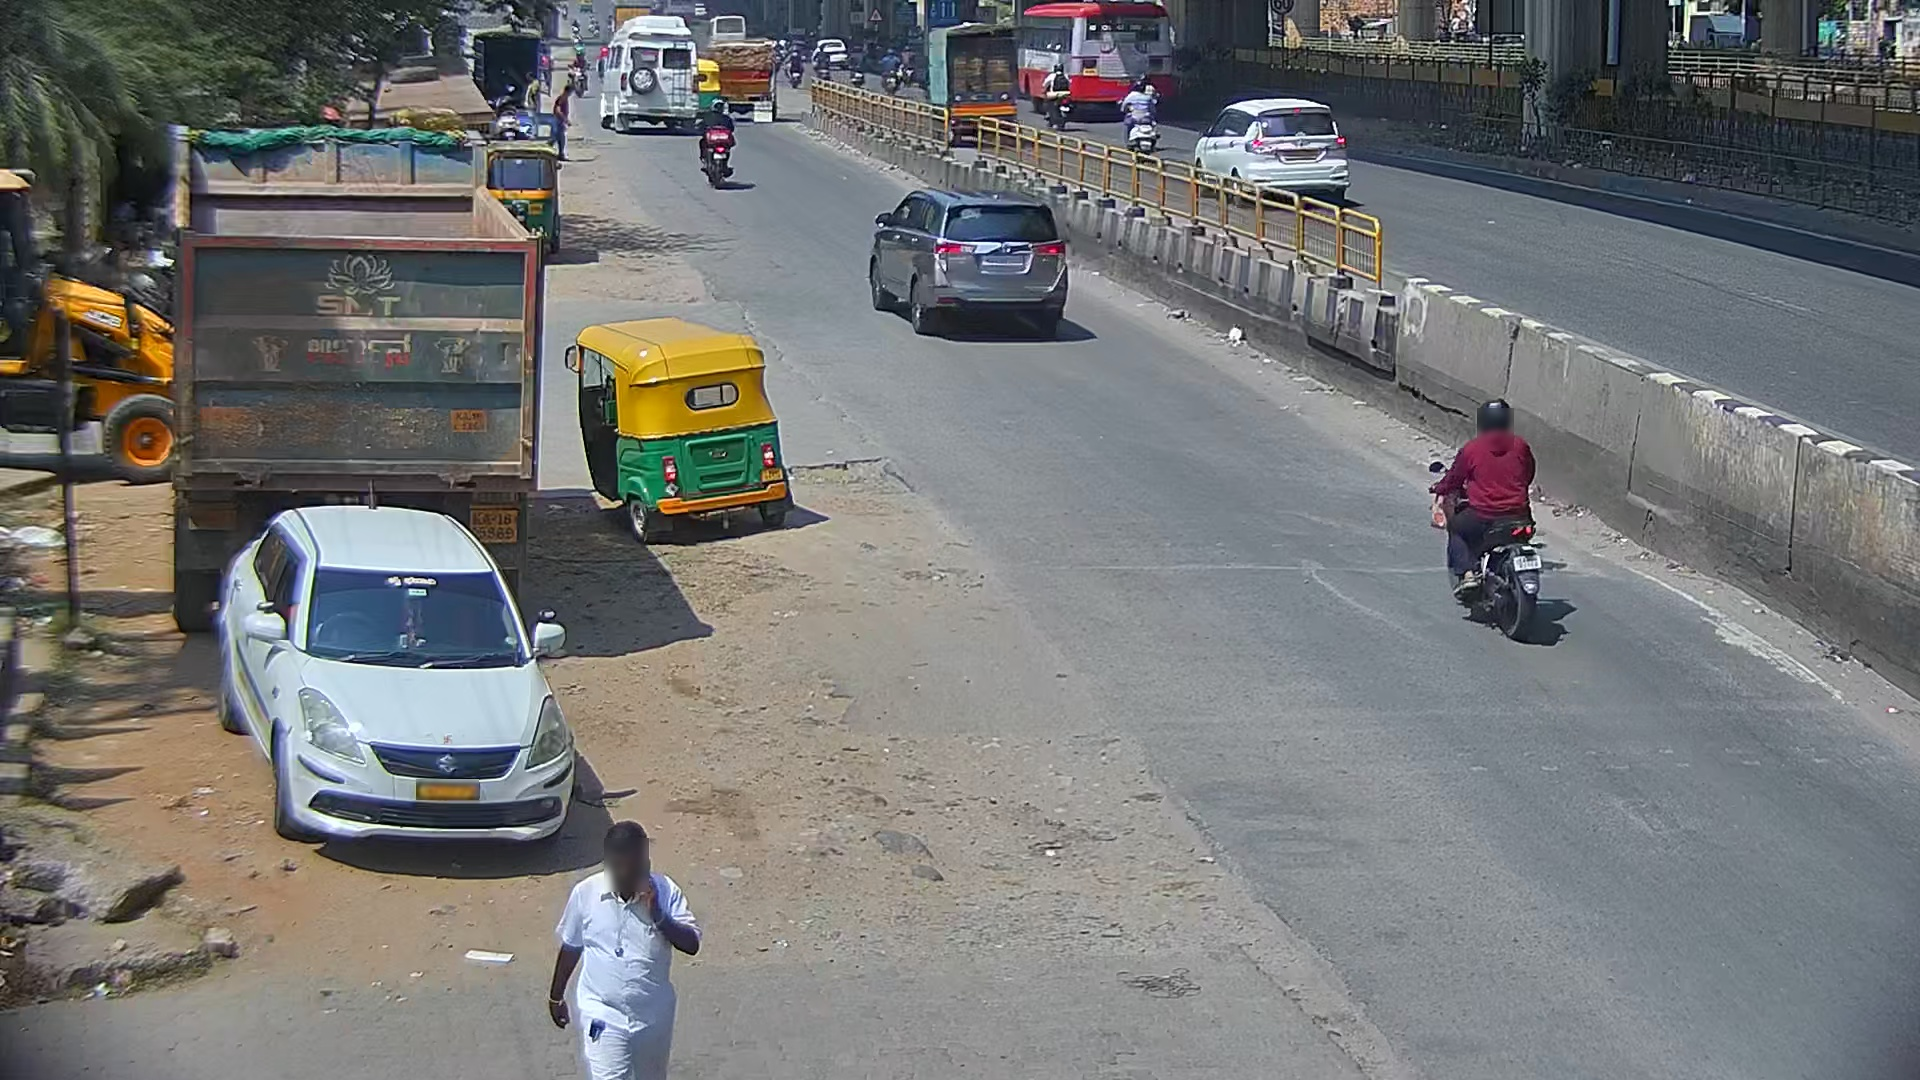
\includegraphics[width=\textwidth]{docs/assets/report/uvh26_val_sample_a.png}
        \caption{Validation sample A}
    \end{subfigure}
    \caption{UVH-26 dataset samples used for distributed viewpoint analytics context.}
    \label{fig:uvh26_samples}
\end{figure}

These samples show typical urban traffic complexity: mixed vehicle classes, partial occlusions, varying depth, and non-uniform density distributions. Such characteristics justify distributed aggregation because per-viewpoint statistics must integrate large numbers of heterogeneous object instances.

\section{Execution Artifacts and Observability}

\subsection{Full-Scale Output Characteristics}
The Stage 2 full artifact contains:
\begin{itemize}
    \item \textbf{Input mapping rows:} 26,646
    \item \textbf{Joined annotation rows:} 316,220
    \item \textbf{Output viewpoint rows:} 4,780
\end{itemize}

These figures indicate non-trivial aggregation volume and viewpoint diversity.

\subsection{Log-Centric Verification}
The engine writes timestamped logs that expose:
\begin{enumerate}
    \item Spark application identity,
    \item master mode and parallelism values,
    \item shuffle partition configuration,
    \item row-count progression through the pipeline,
    \item execution duration.
\end{enumerate}

This log policy supports post-run auditability and aligns with distributed systems observability principles.

\subsection{Smoke-to-Full Hierarchical Validation}
A two-level validation ladder is used:
\begin{itemize}
    \item \textbf{Level 1 smoke run:} 10 viewpoints / 100 images to verify schema, joins, and metric formatting.
    \item \textbf{Level 2 full run:} complete mapping coverage to generate the publishable artifact.
\end{itemize}

Hierarchical validation shortens debugging loops while preserving identical metric semantics across scales.

\section{Stage 3 Analytical Layer: Detailed Structure}

\subsection{Functional Layout}
The dashboard provides:
\begin{enumerate}
    \item KPI cards for global monitoring,
    \item congestion ranking bars,
    \item scatter-based multivariate relationships,
    \item class-ratio comparative plots,
    \item tabular summaries and viewpoint-level deep dives.
\end{enumerate}

\subsection{Filter Hierarchy}
The filtering pipeline is organized as:
\begin{equation}
D' = \{x \in D \mid x.\text{total\_images} \geq \tau_i \land x.\text{entropy} \leq \tau_e\}
\end{equation}
where $\tau_i$ is minimum image threshold and $\tau_e$ is maximum entropy threshold.

\begin{lstlisting}[style=pycode,caption={Stage 3 filter and KPI extraction logic.}]
filtered = df[(df["total_images"] >= min_images) & (df["entropy"] <= max_entropy)].copy()

c1.metric("Viewpoints", f"{len(filtered):,}")
c2.metric("Total Vehicles", f"{int(filtered['total_vehicles'].sum()):,}")
c3.metric("Mean Congestion", f"{filtered['congestion_index'].mean():.4f}")
c4.metric("Mean BBox Density", f"{filtered['avg_bbox_density'].mean():.4f}")
\end{lstlisting}

\subsection{Dashboard Figures}
Figure~\ref{fig:stage3_overview} and Figure~\ref{fig:stage3_deepdive} illustrate the dashboard outputs derived from distributed Stage 2 artifacts.

\begin{figure}[!t]
    \centering
    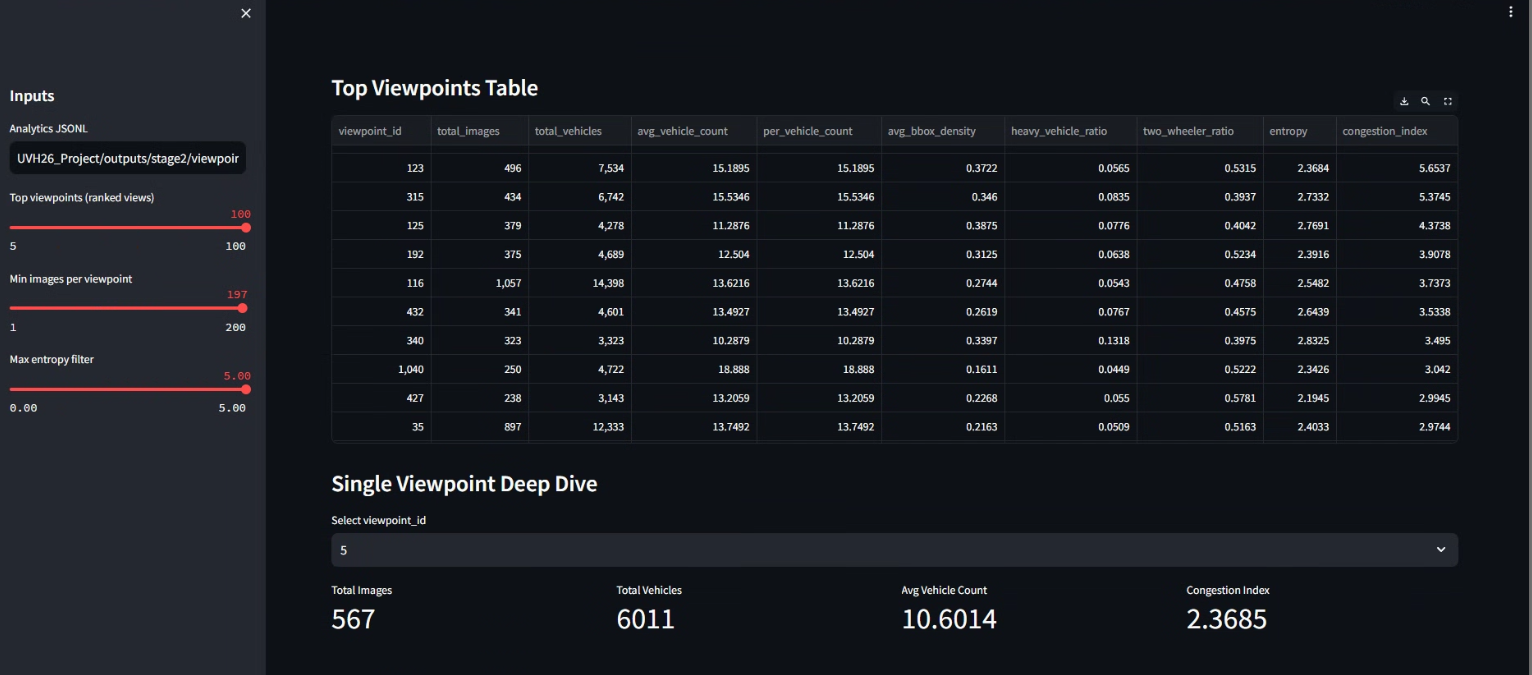
\includegraphics[width=0.95\textwidth]{stage3_dashboard_overview.png}
    \caption{Stage 3 overview: KPI cards, ranking chart, and multidimensional scatter analysis.}
    \label{fig:stage3_overview}
\end{figure}

\begin{figure}[!t]
    \centering
    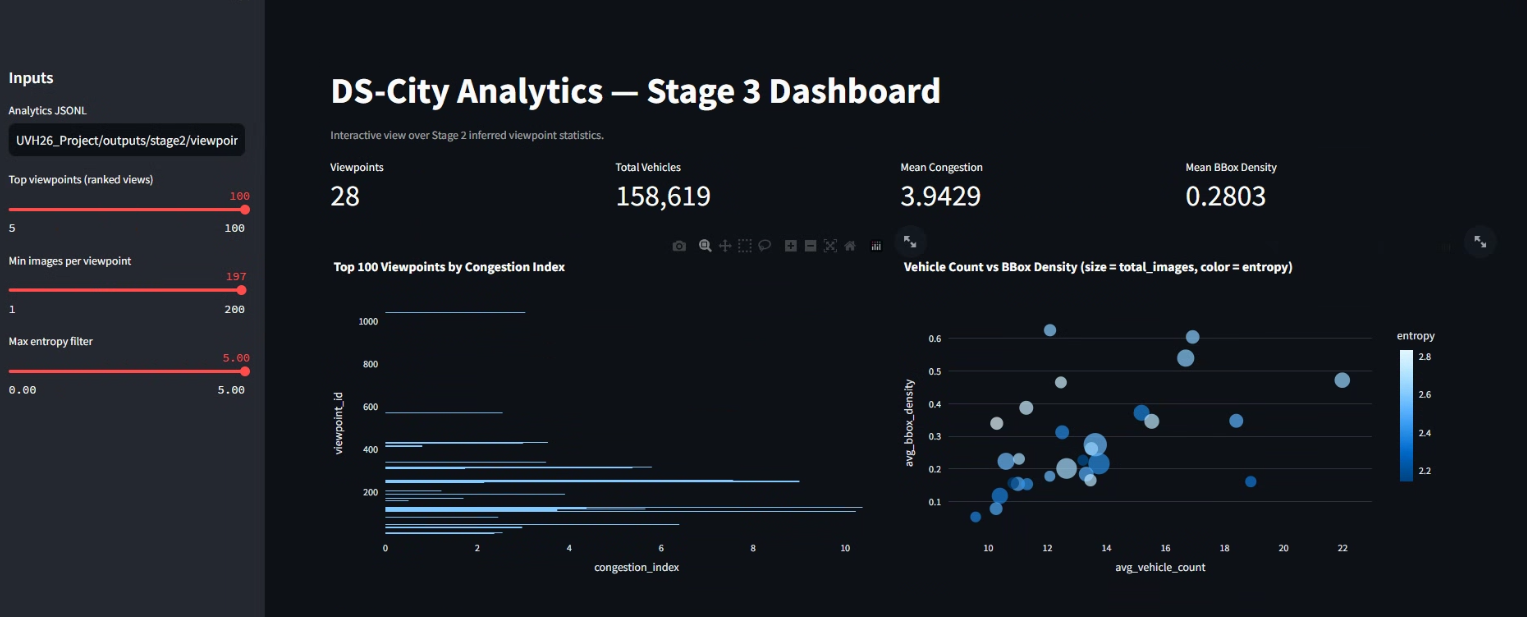
\includegraphics[width=0.95\textwidth]{stage3_dashboard_table_deepdive.png}
    \caption{Stage 3 table and deep-dive panel with per-viewpoint class distribution interpretation.}
    \label{fig:stage3_deepdive}
\end{figure}

\section{Discussion: Distributed Systems Perspective}

\subsection{Why the Pipeline Is Distributed by Design}
The project is distributed by design because core computations are built around partitioned datasets, wide transformations, and reduction operations that naturally map to cluster execution semantics. This includes:
\begin{itemize}
    \item distributed joins between large annotation relations and mapping dimensions,
    \item grouped reductions over thousands of viewpoint keys,
    \item adaptive optimization pathways for shuffle handling.
\end{itemize}

\subsection{Skew Management and Straggler Control}
Skew in viewpoint image counts is a major practical concern. The pre-aggregation bucket assignment strategy reduces heavy-bucket concentration and improves schedule regularity. Additional runtime tuning of shuffle partitions and adaptive execution further mitigates skew impact in wide stages.

\subsection{Failure Handling and Reproducibility}
Spark's lineage model, stage retry mechanisms, and deterministic command-line options provide a reproducible and failure-resilient foundation. The inclusion of preview JSONL outputs and structured logs creates transparent checkpoints between computation and interpretation.

\subsection{Trade-Off Summary}
The implementation prioritizes maintainability and auditability over deeply specialized micro-optimizations. For research-scale and medium-scale city analytics, this trade-off offers high practical value: fast iteration, explicit traceability, and extensibility to new metrics.

\section{Conclusion}

This technical document has detailed a complete distributed viewpoint analytics pipeline over UVH-26, from deterministic mapping construction to distributed metric synthesis and interactive interpretation. The architecture demonstrates that robust traffic intelligence pipelines require explicit handling of data hierarchy, distributed joins, workload balancing, metric formalization, and observability.

The resulting system produces viewpoint-level outputs suitable for hotspot ranking, composition analysis, and uncertainty-aware interpretation. With minimal architectural changes, the same design can support larger city-scale datasets, stronger cluster topologies, and future real-time extensions.

\begin{thebibliography}{12}

\bibitem{sparkdocs}
Apache Spark Project, ``Apache Spark Documentation (Latest),'' 2026. [Online]. Available: \url{https://spark.apache.org/docs/latest/}

\bibitem{sparkstandalone}
Apache Spark Project, ``Spark Standalone Mode,'' 2026. [Online]. Available: \url{https://spark.apache.org/docs/latest/spark-standalone.html}

\bibitem{sparksql}
Apache Spark Project, ``Spark SQL, DataFrames and Datasets Guide,'' 2026. [Online]. Available: \url{https://spark.apache.org/docs/latest/sql-programming-guide.html}

\bibitem{sparktuning}
Apache Spark Project, ``Spark SQL Performance Tuning,'' 2026. [Online]. Available: \url{https://spark.apache.org/docs/latest/sql-performance-tuning.html}

\bibitem{zaharia2016}
M. Zaharia \emph{et al.}, ``Apache Spark: A Unified Engine for Big Data Processing,'' \emph{Communications of the ACM}, vol. 59, no. 11, pp. 56--65, 2016, doi: 10.1145/2934664.

\bibitem{mapreduce}
J. Dean and S. Ghemawat, ``MapReduce: Simplified Data Processing on Large Clusters,'' in \emph{Proc. OSDI}, 2004. [Online]. Available: \url{https://www.usenix.org/conference/osdi-04/mapreduce-simplified-data-processing-large-clusters}

\bibitem{coco}
T.-Y. Lin \emph{et al.}, ``Microsoft COCO: Common Objects in Context,'' arXiv:1405.0312, 2014, doi: 10.48550/arXiv.1405.0312.

\bibitem{shannon1948}
C. E. Shannon, ``A Mathematical Theory of Communication,'' \emph{Bell System Technical Journal}, vol. 27, no. 3, pp. 379--423, 1948, doi: 10.1002/j.1538-7305.1948.tb01338.x.

\bibitem{streamlit}
Streamlit, ``Streamlit Documentation,'' 2026. [Online]. Available: \url{https://docs.streamlit.io/}

\bibitem{plotly}
Plotly Technologies Inc., ``Plotly Open Source Graphing Library for Python,'' 2026. [Online]. Available: \url{https://plotly.com/python/}

\bibitem{submitting}
Apache Spark Project, ``Submitting Applications,'' 2026. [Online]. Available: \url{https://spark.apache.org/docs/latest/submitting-applications.html}

\bibitem{uvh26}
A. Sharma \emph{et al.}, ``Towards Image Annotations and Accurate Vision Models for Indian Traffic, Preliminary Dataset Release, UVH-26-v1.0,'' 2025, doi: 10.48550/arXiv.2511.02563.

\end{thebibliography}

\end{document}
